%-*- program: xelatex -*-        
%-*- program: biber -*-`        
%-*- program: xelatex -*-
\documentclass[11pt]{article}
\usepackage[margin=0.75in]{geometry}            % See geometry.pdf to learn the layout options. There are lots.
\geometry{letterpaper}  
\usepackage{amsmath,textcomp,amssymb,geometry,graphicx,enumerate,upquote,color}
\usepackage{hyperref}
\usepackage{breqn}
\usepackage{float}
\usepackage{tikz}
\usepackage{array}
\usepackage{float}
\usepackage{amsfonts}
\def\Session{Fall 2015}
\usepackage[english]{babel}
\title{Drawdown Project - Risk Contribution}
\author{Boying Gong, Xinyue Zhou}
\newenvironment{qparts}{\begin{enumerate}[{(}a{)}]}{\end{enumerate}}
\def\endproofmark{$\Box$}
\newenvironment{proof}{\par{\bf Proof}:}{\endproofmark\smallskip}
\begin{document}
\maketitle

\tableofcontents

\clearpage

\section{Empirical analysis using two asset class}

In this section, we present the empirical analysis of portfolio risk using two asset class, SPX (S\&P 500 Index) and RMZ (MSCI US REIT Index) in 60/40, 50/50, 40/60 allocation separately. For each portfolio, we calculate the risk contributins of each asset component for CED, ES, VaR and volatility. The four measures indicate similar risk of portfolios over time, but large differences when it comes to risk contributions. The variation of risk contributions for ES, VaR and volatility resemble each other under fixed asset allocation weights. For asset SPX, while the its contribution to ES, VaR and volatility reached its peak during 2010, the contribution of SPX maximized during 2014. Note that in the case of 40/60 asset allocation, SPX contributes to over 98\% of the total CED in 2014. 

Table \ref{table:portfolio_risk} shows how the risk changes for different fixed-mixed portfolios over the period January 3, 2006 to December 31, 2015. ES, VaR and CED are calculated at the 90\% confidence level. RMZ has larger risk than SPX. As we increase the weight of RMZ in the portfolio, the risk indicated by volatility, ES and CED increase. However, VaR of three portfolio are all greater than the individual risk of SPX and RMZ. This result is consistent with the fact that VaR is not sub-additive.

Figure \ref{fig:risk_parity} shows the senario when a protfolio have euqal risk contributions with respect to one risk measure but show difference for other risk measures. We calculated the fractional risk contributions of SPX in two asset profolio in three types of risk parity cases: CED parity, ES parity and volatility parity.

Figure \ref{fig:overall_rc} shows the overall risk contributions of SPX in SPX and RMZ portfolio for weights of 50/50, 60/40 and 70/30. Among the risk measures, VaR shows the greates contribution for SPX and CED the second. As we increase the weight of SPX in the portfolio, the risk contribution increases for all risk measures. 

\begin{figure}[H]
\centering
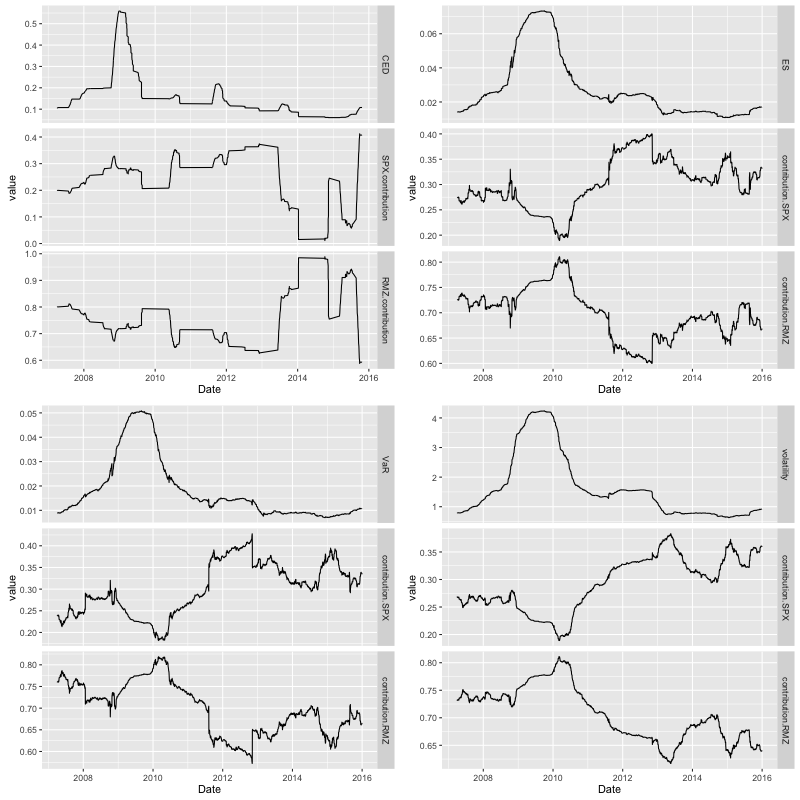
\includegraphics[width = 0.9\textwidth]{../figures/risk_contribution/SPX_RMZ_46}
\caption{3-month 1-year rolling risk contribution for CED, ES, VaR and volatility}
(portfolio is constructed using two asset classes (SPX and RMZ) in the balanced 40/60 allocation, probability level = 0.9)
\label{fig:risk_contribution_SPX_RMZ_46}
\end{figure}

\begin{figure}[H]
\centering
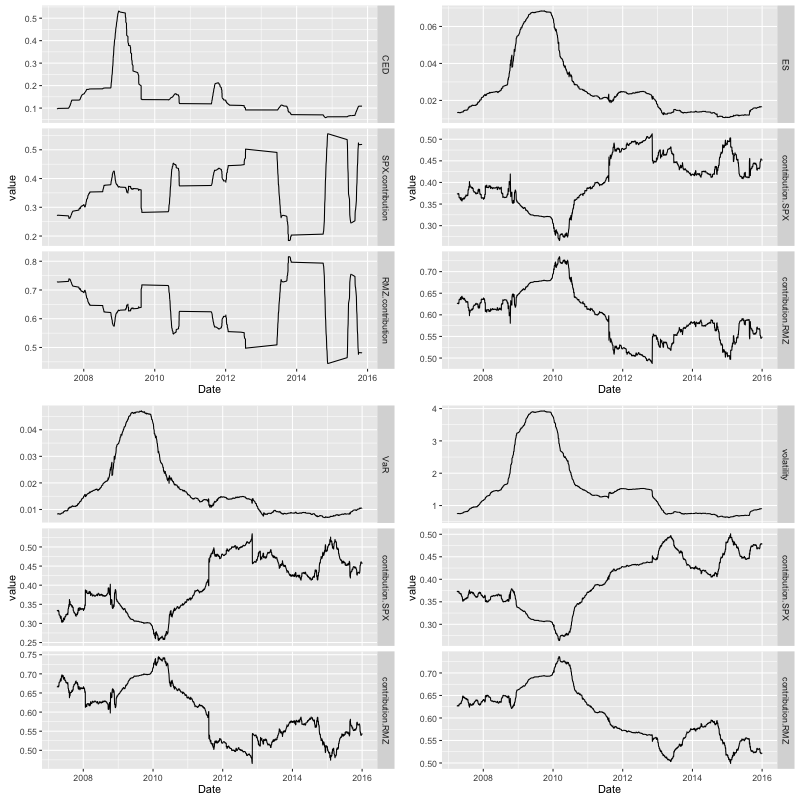
\includegraphics[width = 0.9\textwidth]{../figures/risk_contribution/SPX_RMZ_55}
\caption{3-month 1-year rolling risk contribution for CED, ES, VaR and volatility}
(portfolio is constructed using two asset classes (SPX and RMZ) in the balanced 50/50 allocation, probability level = 0.9)
\label{fig:risk_contribution_SPX_RMZ_55}
\end{figure}

\begin{figure}[H]
\centering
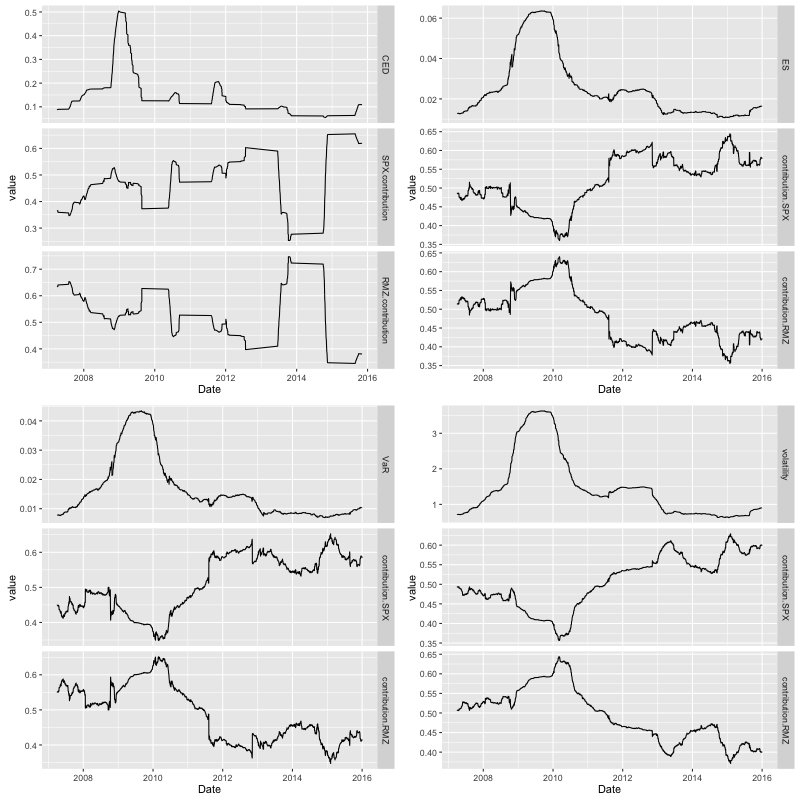
\includegraphics[width = 0.9\textwidth]{../figures/risk_contribution/SPX_RMZ_64}
\caption{3-month 1-year rolling risk contribution for CED, ES, VaR and volatility}
(portfolio is constructed using two asset classes (SPX and RMZ) in the balanced 60/40 allocation, probability level = 0.9)
\label{fig:risk_contribution_SPX_RMZ_64}
\end{figure}

\begin{table}[H]
\centering
\begin{tabular}{r |r r r r r}
\hline
& Volatility & $\textrm{ES}_{0.9}$ & $\textrm{VaR}_{0.9}$ & $\textrm{CED}_{0.9}$ (3-month) & $\textrm{CED}_{0.9}$ (6-month) \\
\hline
\hline
SPX   & 1.31\% & 1.58\% & 0.66\% & 24.79\% & 35.36\%\\
60/40 & 1.63\% & 2.03\% & 0.74\% & 30.00\% & 42.15\%\\
50/50 & 1.74\% & 2.20\% & 0.74\% & 31.49\% & 44.12\%\\ 
40/60 & 1.85\% & 2.39\% & 0.72\% & 32.98\% & 46.10\%\\
RMZ   & 2.35\% & 3.23\% & 0.67\% & 39.54\% & 54.63\%\\
\hline
\end{tabular}
\caption{Risk measures for daily SPX and RMZ and three fixed-mix portfolios over the period January 3, 2006 to December 31, 2015. ES, VaR and CED are calculated at the 90\% confidence level. Three drawdown risk metrics are calculated by considering the maximum drawdown within return paths of different fixed lengths (3 months and 6 month)}
\label{table:portfolio_risk}
\end{table}

\begin{figure}[H]
\centering
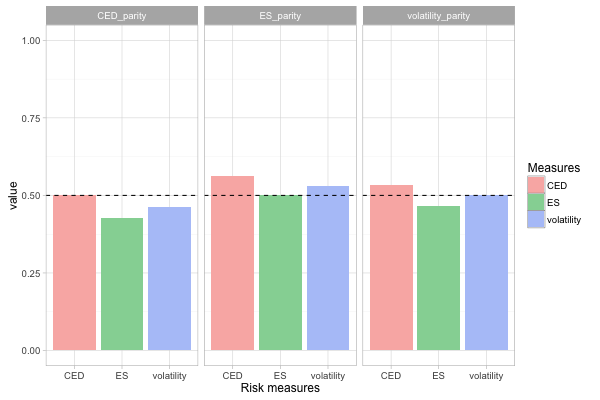
\includegraphics[width = 0.7\textwidth]{../figures/risk_contribution/risk_parity}
\caption{Fractional Risk Contributions of SPX constructed based on CED Parity, ES Parity and Volatility Parity. Protfolios are based on SPX and RMZ over the period January 3, 2006 to December 31, 2015. ES and CED are calculated at the 90\% confidence level. Maximum drawdown distribution is calculated based on 3-month rolling period.}
\label{fig:risk_parity}
\end{figure}

\begin{figure}[H]
\centering
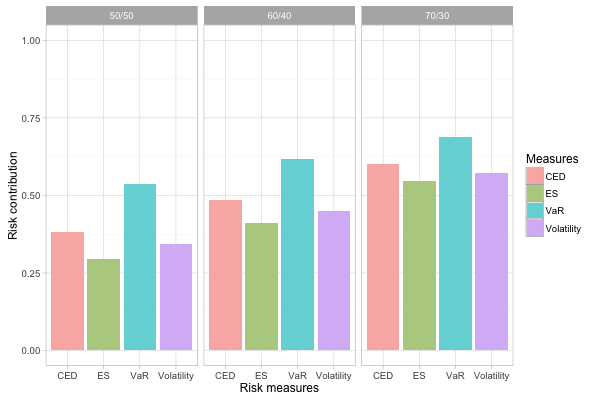
\includegraphics[width = 0.7\textwidth]{../figures/risk_contribution/overall_rc}
\caption{Fractional Risk Contributions of SPX for the weights of 50\%, 60\% and 70\%. Protfolios are based on SPX and RMZ over the period January 3, 2006 to December 31, 2015. ES and CED are calculated at the 90\% confidence level. Maximum drawdown distribution is calculated based on 3-month rolling period.}
\label{fig:overall_rc}
\end{figure}


\end{document}













